\documentclass[11pt]{article}
\usepackage{amsmath, amssymb, physics, mathtools, bm}
\usepackage{tikz, pgfplots}
\pgfplotsset{compat=1.18}
\usetikzlibrary{calc, positioning, decorations.pathmorphing}
\usepackage[margin=2.3cm]{geometry}
\usepackage{siunitx, booktabs, hyperref}
\usepackage{braket}

\newcommand{\D}{\mathrm{D}}
\newcommand{\de}{\mathrm{d}}
\newcommand{\pd}[2]{\frac{\partial #1}{\partial #2}}
\newcommand{\pdd}[2]{\frac{\partial^{2} #1}{\partial #2^{2}}}
\newcommand{\Lap}{\nabla^{2}}

\title{B1 Flows, Fluctuations and Complexity --- Model Solutions, Trinity 2015}
\author{}
\date{}

\begin{document}
\maketitle

\noindent\textit{Navier--Stokes for incompressible viscous flow under gravity:}
\begin{equation}
\pd{\vb u}{t} + (\vb u\cdot\nabla)\vb u + \frac{1}{\rho}\nabla p + g\hat{\vb k} = \nu\Lap\vb u.
\label{eq:NS}
\end{equation}

% =====================================================================
\section*{Question 1 --- 2D velocity decomposition, vorticity, enstrophy}

\textbf{Problem.} Taylor-expand a 2D velocity field about the origin, identify the four kinematic components (translation, divergence, rotation, two strains); discuss dye evolution and the role of molecular diffusion in 2D turbulence; derive the 2D vorticity equation; explain why enstrophy is dissipated.

\subsection*{(a) Taylor expansion and kinematic decomposition}

Taylor-expand $u(x,y)$ and $v(x,y)$ to first order about the origin:
\[ u = u_0 + (\pd{u}{x})_0 x + (\pd{u}{y})_0 y + \cdots, \qquad v = v_0 + (\pd{v}{x})_0 x + (\pd{v}{y})_0 y + \cdots. \]
Write each derivative as the symmetric / antisymmetric combination:
\[ \pd{u}{x} = \tfrac12(D + S_1),\qquad \pd{v}{y} = \tfrac12(D - S_1), \]
\[ \pd{u}{y} = \tfrac12(S_2 - \omega),\qquad \pd{v}{x} = \tfrac12(S_2 + \omega). \]
Substitute into the expansion:
\begin{equation}
\boxed{\;u = u_0 + \tfrac{D}{2}x - \tfrac{\omega}{2}y + \tfrac{S_1}{2}x + \tfrac{S_2}{2}y,\quad v = v_0 + \tfrac{D}{2}y + \tfrac{\omega}{2}x - \tfrac{S_1}{2}y + \tfrac{S_2}{2}x.\;}
\label{eq:decomp}
\end{equation}

Physical interpretation:
\begin{itemize}
  \item $(u_0,v_0)$ --- uniform translation of the parcel.
  \item $D = \nabla\cdot\vb u$ --- isotropic dilation (expansion if $D>0$, contraction if $D<0$).
  \item $\omega$ --- rigid-body rotation about the origin at angular rate $\omega/2$.
  \item $S_1$ --- pure strain along the $x$-axis (stretches $x$, compresses $y$).
  \item $S_2$ --- pure strain along the $45^\circ$ axis (stretches along $y=x$, compresses along $y=-x$).
\end{itemize}

\begin{center}
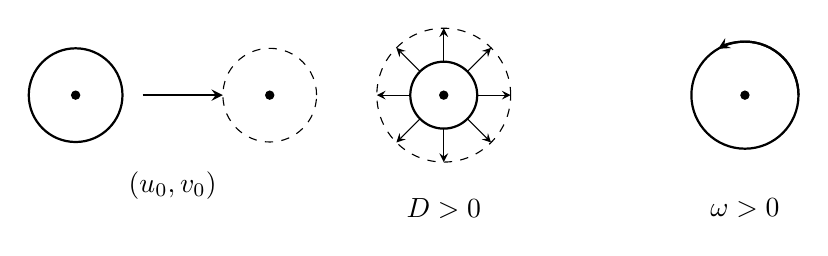
\begin{tikzpicture}[>=stealth, scale=0.85]
  % translation
  \begin{scope}[xshift=0cm]
    \draw[thick] (0,0) circle (0.7);
    \draw[->,thick] (1.0,0) -- (2.2,0);
    \draw[dashed] (2.9,0) circle (0.7);
    \node[circle,fill,inner sep=1.2pt] at (0,0) {};
    \node[circle,fill,inner sep=1.2pt] at (2.9,0) {};
    \node[below] at (1.45,-1.0) {$(u_0,v_0)$};
  \end{scope}
  % divergence
  \begin{scope}[xshift=5.5cm]
    \draw[thick] (0,0) circle (0.5);
    \draw[dashed] (0,0) circle (1.0);
    \foreach \a in {0,45,90,135,180,225,270,315} {\draw[->] (\a:0.5) -- (\a:1.0);}
    \node[circle,fill,inner sep=1.2pt] at (0,0) {};
    \node[below] at (0,-1.4) {$D>0$};
  \end{scope}
  % rotation
  \begin{scope}[xshift=10cm]
    \draw[thick] (0,0) circle (0.8);
    \draw[->, thick] (0.8,0) arc (0:120:0.8);
    \node[circle,fill,inner sep=1.2pt] at (0,0) {};
    \node[below] at (0,-1.4) {$\omega>0$};
  \end{scope}
\end{tikzpicture}
\end{center}
\begin{center}
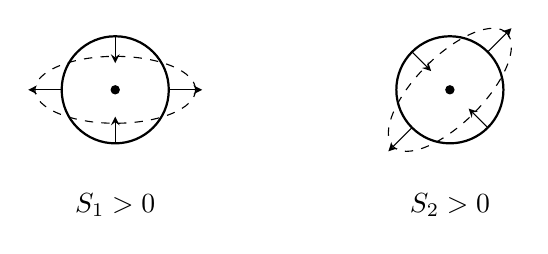
\begin{tikzpicture}[>=stealth, scale=0.85]
  % S1 strain
  \begin{scope}[xshift=0cm]
    \draw[thick] (0,0) circle (0.8);
    \draw[dashed] (0,0) ellipse (1.2 and 0.5);
    \draw[->] (0.8,0) -- (1.3,0); \draw[->] (-0.8,0) -- (-1.3,0);
    \draw[->] (0,0.8) -- (0,0.4); \draw[->] (0,-0.8) -- (0,-0.4);
    \node[circle,fill,inner sep=1.2pt] at (0,0) {};
    \node[below] at (0,-1.4) {$S_1>0$};
  \end{scope}
  % S2 strain
  \begin{scope}[xshift=5cm]
    \draw[thick] (0,0) circle (0.8);
    \draw[dashed,rotate=45] (0,0) ellipse (1.2 and 0.5);
    \draw[->] (0.566,0.566) -- (0.92,0.92); \draw[->] (-0.566,-0.566) -- (-0.92,-0.92);
    \draw[->] (-0.566,0.566) -- (-0.28,0.28); \draw[->] (0.566,-0.566) -- (0.28,-0.28);
    \node[circle,fill,inner sep=1.2pt] at (0,0) {};
    \node[below] at (0,-1.4) {$S_2>0$};
  \end{scope}
\end{tikzpicture}
\end{center}

\subsection*{(b) Dye evolution in 2D incompressible turbulence}

Incompressibility: $D=0$, so the parcel area is preserved. Local flow is rotation $+ $ pure strain. Strain stretches the parcel exponentially along one principal axis and compresses it along the perpendicular axis at the same rate (area-preserving); rotation reorients the principal axes as the parcel is advected through the random strain field.

\begin{center}
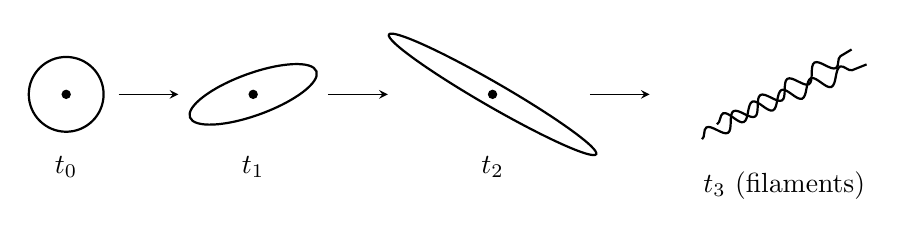
\begin{tikzpicture}[>=stealth, scale=0.95]
  \draw[thick] (0,0) circle (0.5);
  \node[circle,fill,inner sep=1.2pt] at (0,0) {};
  \node[below] at (0,-0.7) {$t_0$};
  \draw[->] (0.7,0) -- (1.5,0);
  \draw[thick, rotate around={20:(2.5,0)}] (2.5,0) ellipse (0.9 and 0.28);
  \node[circle,fill,inner sep=1.2pt] at (2.5,0) {};
  \node[below] at (2.5,-0.7) {$t_1$};
  \draw[->] (3.5,0) -- (4.3,0);
  \draw[thick, rotate around={-30:(5.7,0)}] (5.7,0) ellipse (1.6 and 0.16);
  \node[circle,fill,inner sep=1.2pt] at (5.7,0) {};
  \node[below] at (5.7,-0.7) {$t_2$};
  \draw[->] (7.0,0) -- (7.8,0);
  \draw[thick, decorate, decoration={snake, segment length=4mm, amplitude=1mm}] (8.5,-0.6) -- (10.5,0.6);
  \draw[thick, decorate, decoration={snake, segment length=4mm, amplitude=1mm}] (8.7,-0.4) -- (10.7,0.4);
  \node[below] at (9.6,-0.9) {$t_3$ (filaments)};
\end{tikzpicture}
\end{center}

The parcel becomes an exponentially thinning, lengthening filament. Once the filament thickness reaches the diffusive cutoff $\ell_d \sim \sqrt{\kappa\tau}$ (where $\kappa$ is the molecular diffusivity and $\tau$ the strain time), the dye gradient $\nabla c \sim c/\ell_d$ becomes large enough that molecular diffusion $\kappa\Lap c$ smooths the field at the same rate as straining produces gradients --- diffusion cannot be neglected, and dye is mixed irreversibly even though the underlying flow is reversible.

\subsection*{(c) 2D vorticity equation}

Take the curl of \eqref{eq:NS} (gravity drops, $\nabla\cdot\vb u=0$). For 2D flow $\vb u=(u,v,0)$, vorticity $\bm\omega=\omega\hat{\vb z}$ with $\omega = \partial_x v - \partial_y u$. Apply $\partial_y$ to the $x$-NS, $\partial_x$ to the $y$-NS, subtract:
\[ \pd{}{t}(\partial_x v - \partial_y u) + \partial_x[(u\cdot\nabla)v] - \partial_y[(u\cdot\nabla)u] = \nu\Lap(\partial_x v - \partial_y u). \]
Expand the advective terms:
\[ \partial_x[u\partial_x v + v\partial_y v] - \partial_y[u\partial_x u + v\partial_y u]. \]
Use $\partial_x u + \partial_y v = 0$ to cancel cross terms:
\[ = u\partial_x\omega + v\partial_y\omega. \]
Collect:
\begin{equation}
\boxed{\;\left(\pd{}{t} + u\pd{}{x} + v\pd{}{y}\right)\omega = \nu\Lap\omega.\;}
\label{eq:vort2D}
\end{equation}

High-Re limit ($\nu\to 0$):
\begin{equation}
\boxed{\;\frac{\D\omega}{\D t} = 0.\;}
\label{eq:vortInv}
\end{equation}
Vorticity is materially conserved; in 2D there is no vortex stretching.

\subsection*{(d) Enstrophy is always dissipated}

Multiply \eqref{eq:vort2D} by $\omega$, integrate over the (unbounded or no-flux) domain. Advective term integrates to zero by incompressibility:
\[ \pd{}{t}\iint \tfrac{\omega^2}{2}\,\de x\,\de y = \nu\iint \omega\Lap\omega\,\de x\,\de y. \]
Integrate by parts (boundary terms vanish):
\[ = -\nu\iint |\nabla\omega|^2\,\de x\,\de y \le 0. \]
Stretching strains thin vorticity filaments, increasing $|\nabla\omega|$, so the dissipation rate grows even as $\nu\to 0$. Hence enstrophy decays monotonically in 2D turbulence:
\[ \boxed{\;\pd{}{t}\iint \tfrac{\omega^2}{2}\,\de x\,\de y = -\nu\iint|\nabla\omega|^2\,\de x\,\de y \le 0.\;} \]

% =====================================================================
\section*{Question 2 --- Sound waves, Riemann invariants, shocks}

\textbf{Problem.} From 1D adiabatic compressible Euler-with-viscosity, linearise to obtain $c=\sqrt{\partial p/\partial \rho}$; recast nonlinear inviscid form as Riemann invariants on characteristics; write the implicit simple-wave solution, sketch wave steepening, and estimate the shock thickness $\delta\sim\nu/c$.

\subsection*{(a) Linearisation and sound speed}

Inviscid limit: $\nu=0$. Perturb about rest:
\[ u = u', \quad \rho = \rho_0 + \rho', \quad p = p_0 + p',\qquad \rho',p',u'\ll. \]
Linearise momentum (drop $u\partial_x u$):
\[ \pd{u'}{t} + \frac{1}{\rho_0}\pd{p'}{x} = 0. \]
Linearise continuity:
\[ \pd{\rho'}{t} + \rho_0\pd{u'}{x} = 0. \]
Adiabatic state law: $p = p_0(\rho/\rho_0)^\gamma$. Differentiate:
\[ \pd{p}{\rho} = \gamma p_0\rho_0^{-\gamma}\rho^{\gamma-1}, \]
At rest:
\[ \left.\pd{p}{\rho}\right|_0 = \frac{\gamma p_0}{\rho_0}. \]
So $p' = (\gamma p_0/\rho_0)\rho'$. Eliminate $\rho'$:
\[ \pdd{u'}{t} - \frac{\gamma p_0}{\rho_0}\pdd{u'}{x} = 0. \]
Wave equation, speed:
\begin{equation}
\boxed{\;c = \sqrt{\pd{p}{\rho}} = \sqrt{\frac{\gamma p_0}{\rho_0}}.\;}
\label{eq:c}
\end{equation}

Numerical estimate at sea level: $\gamma=7/5$, $p_0=\SI{e5}{Pa}$, $\rho_0=\SI{1.2}{kg.m^{-3}}$:
\[ \gamma p_0 = 1.4 \times 10^5 = \SI{1.4e5}{Pa}. \]
\[ \frac{\gamma p_0}{\rho_0} = \frac{1.4\times 10^5}{1.2} = \SI{1.17e5}{m^2.s^{-2}}. \]
\[ c = \sqrt{1.17\times 10^5} \approx \SI{342}{m.s^{-1}}. \]
\[ \boxed{\;c \approx \SI{340}{m.s^{-1}}.\;} \]

\subsection*{(b) Riemann invariants}

Write momentum (inviscid) and continuity:
\[ \pd{u}{t} + u\pd{u}{x} + \frac{1}{\rho}\pd{p}{x} = 0,\qquad \pd{\rho}{t} + u\pd{\rho}{x} + \rho\pd{u}{x} = 0. \]
Use $p=p(\rho)$, so $\partial_x p = c^2\partial_x\rho$, and $\de P = \de p/(\rho c)$ implies $\partial_x P = (c/\rho)\partial_x\rho$ and $\partial_t P = (c/\rho)\partial_t\rho$. Rewrite continuity:
\[ \pd{P}{t} + u\pd{P}{x} + c\pd{u}{x} = 0. \]
Rewrite momentum (using $\partial_x p/\rho = c\,\partial_x P$):
\[ \pd{u}{t} + u\pd{u}{x} + c\pd{P}{x} = 0. \]
Add the two:
\[ \pd{}{t}(u+P) + (u+c)\pd{}{x}(u+P) = 0. \]
Subtract:
\[ \pd{}{t}(u-P) + (u-c)\pd{}{x}(u-P) = 0. \]
\begin{equation}
\boxed{\;\left[\pd{}{t}+(u+c)\pd{}{x}\right](u+P)=0,\quad \left[\pd{}{t}+(u-c)\pd{}{x}\right](u-P)=0.\;}
\label{eq:Riemann}
\end{equation}

\subsection*{(c) Simple wave, shock formation, shock thickness}

For a wave moving in $+x$ relative to mean flow, take $u-P=$ const everywhere (uniform upstream); then $P = u + $ const, so $u+P = 2u+$ const is constant on $C_+$ characteristics $\de x/\de t = u+c$. Hence $u$ itself is constant along $C_+$:
\begin{equation}
\boxed{\;u(x,t) = u_0\!\left(x - (u+c)t\right),\;}
\label{eq:simple}
\end{equation}
implicit because the characteristic speed depends on $u$.

\begin{center}
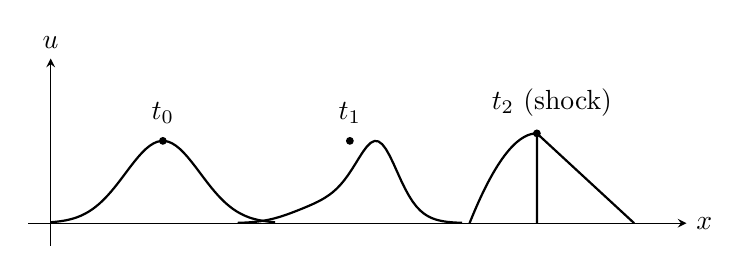
\begin{tikzpicture}[>=stealth, scale=0.95]
  \draw[->] (-0.3,0) -- (8.5,0) node[right] {$x$};
  \draw[->] (0,-0.3) -- (0,2.2) node[above] {$u$};
  % t0: smooth bump
  \draw[thick] plot[domain=0:3, samples=60] (\x, {1.1*exp(-(\x-1.5)^2/0.5)});
  \node[above] at (1.5,1.2) {$t_0$};
  % t1: leaning forward
  \draw[thick] plot[domain=2.5:5.5, samples=60] (\x, {1.1*exp(-(\x-4.0-0.4*1.1*exp(-(\x-4.0)^2/0.5))^2/0.4)});
  \node[above] at (4.0,1.2) {$t_1$};
  % t2: vertical front (shock)
  \draw[thick] (6.5,0) -- (6.5,1.2) -- (7.8,0);
  \draw[thick] (5.6,0) .. controls (6.0,1.0) and (6.3,1.2) .. (6.5,1.2);
  \node[above] at (6.7,1.3) {$t_2$ (shock)};
  \node[circle,fill,inner sep=1pt] at (1.5,1.1) {};
  \node[circle,fill,inner sep=1pt] at (4.0,1.1) {};
  \node[circle,fill,inner sep=1pt] at (6.5,1.2) {};
\end{tikzpicture}
\end{center}

Crests (large $u$) travel faster than troughs ($u+c$ depends on $u$); the wave leans forward and steepens until $\partial_x u\to-\infty$. Inviscid theory gives a multi-valued solution, unphysical: viscosity smooths the front, producing a thin shock.

Shock-thickness estimate: in the shock, balance the inertial term $u\partial_x u$ against the viscous term $\nu\partial_x^2 u$. Take $u\sim c$ (transonic) and $\partial_x \sim 1/\delta$:
\[ u\pd{u}{x} \sim \frac{c^2}{\delta}, \]
\[ \nu\pdd{u}{x} \sim \frac{\nu c}{\delta^2}. \]
Equate:
\[ \frac{c^2}{\delta} \sim \frac{\nu c}{\delta^2}. \]
Solve:
\begin{equation}
\boxed{\;\delta \sim \frac{\nu}{c}.\;}
\label{eq:shockwidth}
\end{equation}

Numerical estimate at sea level: $\nu = \SI{1.5e-5}{m^2.s^{-1}}$, $c=\SI{340}{m.s^{-1}}$:
\[ \delta \sim \frac{1.5\times 10^{-5}}{340}. \]
\[ \delta \sim \SI{4.4e-8}{m}. \]
\[ \boxed{\;\delta \sim \SI{4e-8}{m} \sim 100\,\text{atomic spacings}.\;} \]
Comparable to molecular mean free path; continuum description marginal.

% =====================================================================
\section*{Question 3 --- Phase-space dynamics and a strange attractor}

\textbf{Problem.} For $\dot x = yz,\ \dot y = x-y,\ \dot z = 1-xy$: locate fixed points and prove instability; derive the phase-space continuity equation and show $\delta V = \delta V_0 e^{-(t-t_0)}$; show $\|\delta\vb x\|=\|\delta\vb x\|_0 e^{\lambda t}$ along an eigendirection of $(J+J^T)/2$; compute those eigenvalues at the origin; discuss the attractor's geometry.

\subsection*{(a) Fixed points and stability}

Fixed points: $\dot x=\dot y=\dot z=0$:
\[ yz = 0,\qquad x = y,\qquad xy = 1. \]
$xy=1$ rules out $y=0$, so $z=0$ and $x=y=\pm 1$:
\[ \boxed{\;\vb x_\pm = (\pm 1,\pm 1,0).\;} \]

Jacobian:
\[ J = \begin{pmatrix} 0 & z & y \\ 1 & -1 & 0 \\ -y & -x & 0 \end{pmatrix}. \]
At $\vb x_+=(1,1,0)$:
\[ J_+ = \begin{pmatrix} 0 & 0 & 1 \\ 1 & -1 & 0 \\ -1 & -1 & 0 \end{pmatrix}. \]
Characteristic polynomial $\det(J_+-r I)=0$. Compute:
\[ \det\begin{pmatrix} -r & 0 & 1 \\ 1 & -1-r & 0 \\ -1 & -1 & -r \end{pmatrix}. \]
Expand along the top row:
\[ -r[(-1-r)(-r) - 0] + 1\cdot[1\cdot(-1) - (-1-r)(-1)]. \]
Simplify:
\[ -r[r(1+r)] + [-1 - (1+r)]. \]
\[ -r^3 - r^2 - 2 - r. \]
Multiply by $-1$ to standard form $r^3+Ar^2+Br+C=0$:
\[ r^3 + r^2 + r + 2 = 0. \]
Read off: $A=1,\ B=1,\ C=2$. All positive. Test $C>AB$:
\[ 2 > 1\cdot 1 = 1\quad\checkmark. \]
By the stated criterion, $\vb x_+$ has at least one root with positive real part.

By the symmetry $(x,y)\to(-x,-y)$, $z\to z$ (which leaves the system invariant), $\vb x_-$ has the same characteristic polynomial. \emph{Both fixed points are unstable.}

\subsection*{(b) Phase-space continuity and volume contraction}

For $\dot{\vb x}=\vb f(\vb x)$, the phase-space density $n(\vb x,t)$ obeys:
\[ \pd{n}{t} + \nabla\cdot(n\vb f) = 0. \]
Apply to a comoving volume element $\delta V$ containing fixed phase points. Conservation of points:
\[ n\,\delta V = \text{const} \;\Rightarrow\; \frac{1}{\delta V}\frac{\D \delta V}{\D t} = -\frac{1}{n}\frac{\D n}{\D t}. \]
Use the continuity equation along a streamline:
\[ \frac{\D n}{\D t} = -n\,\nabla\cdot\vb f. \]
Combine:
\[ \frac{\D \delta V}{\D t} = (\nabla\cdot\vb f)\,\delta V. \]
Compute the divergence:
\[ \nabla\cdot\vb f = \pd{}{x}(yz) + \pd{}{y}(x-y) + \pd{}{z}(1-xy) = 0 - 1 + 0 = -1. \]
Solve:
\begin{equation}
\boxed{\;\delta V(t) = \delta V_0\,e^{-(t-t_0)}.\;}
\label{eq:volcontract}
\end{equation}

Volume contracts at constant rate. Trajectories are bounded (numerical evidence) yet repelled by both fixed points and not converging to one --- so they collapse onto a zero-volume invariant set. That set is either a one-dimensional limit cycle or, if local stretching coexists with global contraction, a fractal-dimensional \emph{strange attractor}.

\subsection*{(c) Symmetric-Jacobian growth rate and eigenvalues at origin}

Linearise: $\delta\dot{\vb x} = J\,\delta\vb x$. Squared length:
\[ \frac{\de}{\de t}\|\delta\vb x\|^2 = 2\,\delta\vb x\cdot J\,\delta\vb x. \]
Symmetrise the inner product:
\[ 2\,\delta\vb x\cdot J\,\delta\vb x = \delta\vb x\cdot(J+J^T)\,\delta\vb x. \]
Choose $\delta\vb x$ aligned with eigenvector of $(J+J^T)/2$ with eigenvalue $\lambda$:
\[ \frac{\de}{\de t}\|\delta\vb x\|^2 = 2\lambda\|\delta\vb x\|^2. \]
Integrate (treating $J$ as locally constant for short $t$):
\begin{equation}
\boxed{\;\|\delta\vb x\| = \|\delta\vb x\|_0\,e^{\lambda(t-t_0)}.\;}
\label{eq:symstretch}
\end{equation}

At the origin, $J(0,0,0) = \begin{pmatrix}0&0&0\\1&-1&0\\0&0&0\end{pmatrix}$:
\[ \frac{J+J^T}{2} = \begin{pmatrix} 0 & 1/2 & 0 \\ 1/2 & -1 & 0 \\ 0 & 0 & 0 \end{pmatrix}. \]
$z$-direction decouples: $\lambda_3 = 0$. For the $(x,y)$ block:
\[ \det\!\begin{pmatrix}-\lambda & 1/2 \\ 1/2 & -1-\lambda\end{pmatrix}=0. \]
Expand:
\[ \lambda(1+\lambda) - 1/4 = 0. \]
\[ \lambda^2 + \lambda - 1/4 = 0. \]
Quadratic formula:
\[ \lambda = \frac{-1\pm\sqrt{1+1}}{2}. \]
\[ \boxed{\;\lambda \in \left\{\,\tfrac{-1+\sqrt 2}{2},\ \tfrac{-1-\sqrt 2}{2},\ 0\,\right\} \approx \{+0.207,\ -1.207,\ 0\}.\;} \]

\subsection*{(d) Geometry of the attractor}

\textit{Discussion.} Fractal dimension $D_f\approx 2.174$ lies between 2 and 3: the attractor is a sheet-like object with a fine, self-similar transverse structure --- consistent with continual local stretching plus folding.

The volume-contraction result \eqref{eq:volcontract} shows phase-space volumes shrink at rate $1$, so the sum of Lyapunov exponents is $\sum\lambda_i = -1$. From \eqref{eq:symstretch} the symmetric-part eigenvalues at the origin are $+0.207$, $0$, $-1.207$; their sum is $-1$, matching the trace. Local stretching ($\lambda_+>0$) coexists with strong contraction ($\lambda_-<0$), the hallmark of a strange attractor: nearby trajectories diverge along the $\lambda_+$ axis while the volume collapses along $\lambda_-$, producing a fractal sheet. The two unstable fixed points $\vb x_\pm$ act as scrolling centres: the trajectory loops around one, ejects, and is captured by the other, building the two-lobed structure visible in the figure (qualitatively similar to a Lorenz-like attractor).

The Kaplan--Yorke estimate $D_f = 2 + \lambda_+/|\lambda_-|$ gives, with the symmetric-Jacobian numbers, $D_f \approx 2 + 0.207/1.207 \approx 2.17$, consistent with the quoted $2.174$ (true Lyapunov exponents would be needed for an exact match, but the agreement supports the strange-attractor identification).

% =====================================================================
\section*{Question 4 --- Freely-jointed chains, loop closure, DNA looping}

\textbf{Problem.} Find the most-probable end-to-end distance for an unconfined Gaussian FJC and for one tethered to a wall; obtain $S(z)$. Compute the loop-closure entropy $\Delta S = B - \tfrac32 k_B\ln N$; combine with the elastic loop energy to obtain the DNA loop free energy and find the optimal loop size; choose between Lac-repressor sites at $92$ and $401$ bp.

\subsection*{(a) Most-probable end-to-end distance, untethered FJC}

Joint density:
\[ P(\vb r) = \left(\frac{3}{2\pi N b^2}\right)^{3/2}\exp\!\left(-\frac{3 r^2}{2N b^2}\right). \]
Radial distribution:
\[ p(r) = 4\pi r^2 P(\vb r). \]
Maximise:
\[ \frac{\de}{\de r}\!\left[r^2\exp\!\left(-\frac{3r^2}{2Nb^2}\right)\right] = 0. \]
Differentiate:
\[ 2r - r^2\,\frac{3r}{Nb^2} = 0. \]
Solve:
\[ r_{\rm mp}^2 = \frac{2Nb^2}{3}. \]
\begin{equation}
\boxed{\;r_{\rm mp} = b\sqrt{\frac{2N}{3}}.\;}
\label{eq:rmpfree}
\end{equation}

\subsection*{(b) Tethered FJC: most-probable distance and entropy}

Joint density:
\[ P(\vb r) = P_x(x)P_y(y)\,\frac{z}{\Omega}\exp\!\left(-\frac{3z^2}{2Nb^2}\right),\quad z>0. \]
Maximise $P(\vb r)$ over $(x,y,z)$ directly (not the radial form: the wall breaks isotropy). Gaussian factors $P_x,P_y$ peak at $x=y=0$:
\[ x_{\rm mp} = 0,\qquad y_{\rm mp}=0. \]
Maximise $z\exp(-3z^2/2Nb^2)$:
\[ \frac{\de}{\de z}\!\left[z\exp\!\left(-\frac{3z^2}{2Nb^2}\right)\right] = 0. \]
Differentiate:
\[ 1 - \frac{3z^2}{Nb^2} = 0. \]
Solve:
\[ z_{\rm mp} = b\sqrt{\frac{N}{3}}. \]
At the maximum $r=z$:
\begin{equation}
\boxed{\;r_{\rm mp}^{\rm tethered} = b\sqrt{\frac{N}{3}}.\;}
\label{eq:rmptether}
\end{equation}

\textit{Comment.} Smaller than \eqref{eq:rmpfree} by $\sqrt 2$: the wall removes the radial $4\pi r^2$ phase-space factor (which favoured larger $r$ for the free chain) and replaces it with the linear $z$ factor (only one direction available), so the most probable separation is reduced.

Entropy along $z$:
\[ S(z) = k_B\ln P(z). \]
Substitute $P_z$:
\[ S(z) = k_B\ln\!\left(\frac{z}{\Omega}\right) - \frac{3 k_B z^2}{2 N b^2}. \]
\begin{equation}
\boxed{\;S(z) = k_B\ln\!\left(\frac{z}{\Omega}\right) - \frac{3 k_B z^2}{2 N b^2}.\;}
\label{eq:Sz}
\end{equation}

\begin{center}
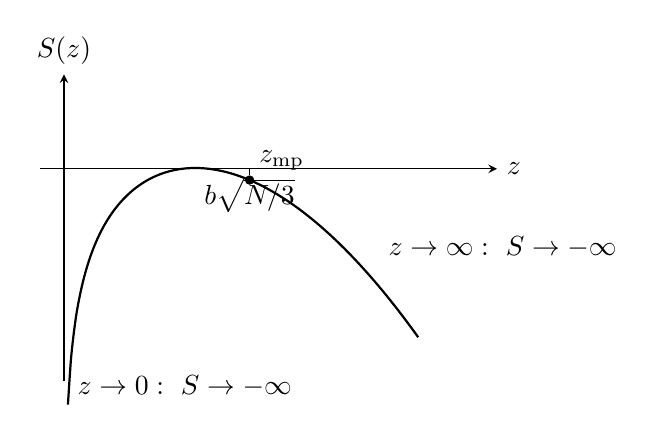
\begin{tikzpicture}[>=stealth, scale=1.0]
  \draw[->] (-0.3,0) -- (5.5,0) node[right] {$z$};
  \draw[->] (0,-2.7) -- (0,1.2) node[above] {$S(z)$};
  % S(z) = ln(z) - z^2 (units chosen so peak at z=sqrt(1/2)?)
  % Use S = ln(z) - 0.5 z^2 ; peak at z=1; at z=0.05, ln(0.05)=-3
  \draw[thick, domain=0.05:4.5, samples=120, smooth] plot (\x, {ln(\x) - 0.18*\x*\x});
  \node[circle,fill,inner sep=1.2pt] (P) at (2.357, {ln(2.357) - 0.18*2.357*2.357}) {};
  \node[above right] at (P) {$z_{\rm mp}$};
  \draw[dashed] (2.357,0) -- (P);
  \node[below] at (2.357,0) {$b\sqrt{N/3}$};
  \node[below right] at (0.05,-2.5) {$z\to 0:\ S\to-\infty$};
  \node[right] at (4.0,-1.0) {$z\to\infty:\ S\to-\infty$};
\end{tikzpicture}
\end{center}

\textit{Comment.} $S\to-\infty$ as $z\to 0$ (only one configuration: chain crushed against wall) \emph{and} as $z\to\infty$ (rare large excursion of a Gaussian). Maximum at $z_{\rm mp}=b\sqrt{N/3}$, agreeing with the most-probable-distance calculation above. Stretching the chain away from $z_{\rm mp}$ reduces entropy and produces a restoring elastic force --- the entropic origin of polymer elasticity.

\subsection*{(c) Loop-closure entropy}

Density of $r=|\vb r|$ for the free chain:
\[ p(r)=4\pi r^2\!\left(\frac{3}{2\pi N b^2}\right)^{3/2}\exp\!\left(-\frac{3r^2}{2Nb^2}\right). \]
Limit $\delta\ll b$ (so $\delta\ll b\sqrt{N}$): exponential $\approx 1$:
\[ \Pi(\delta) \approx 4\pi\!\left(\frac{3}{2\pi N b^2}\right)^{3/2}\!\int_0^\delta r^2\,\de r. \]
Integrate:
\[ \Pi(\delta) \approx \frac{4\pi\delta^3}{3}\!\left(\frac{3}{2\pi Nb^2}\right)^{3/2}. \]
\begin{equation}
\boxed{\;\Pi(\delta) = \frac{4\pi}{3}\!\left(\frac{3}{2\pi}\right)^{3/2}\!\left(\frac{\delta}{b}\right)^{3}N^{-3/2}.\;}
\label{eq:Pi}
\end{equation}

Joining the ends restricts the configurational space from "all $\vb r$" to "$|\vb r|<\delta$". The fractional volume retained is $\Pi(\delta)$. Boltzmann's $S=k_B\ln\Omega$ for fewer accessible states gives $\Delta S = k_B\ln\Pi(\delta)$ (entropy \emph{loss}, $\Delta S<0$).

Take the log:
\[ \Delta S = k_B\ln\!\left[\frac{4\pi}{3}\!\left(\frac{3}{2\pi}\right)^{3/2}\!\left(\frac{\delta}{b}\right)^{3}\right] - \frac{3}{2}k_B\ln N. \]
\begin{equation}
\boxed{\;\Delta S = B - \tfrac{3}{2}k_B\ln N,\qquad B = k_B\ln\!\left[\frac{4\pi}{3}\!\left(\frac{3}{2\pi}\right)^{3/2}\!\left(\frac{\delta}{b}\right)^{3}\right].\;}
\label{eq:DeltaS}
\end{equation}

\subsection*{(d) DNA loop free energy and Lac-repressor choice}

A DNA segment of $n$ base pairs has contour length $L_c = nL$ with $L=\SI{0.34}{nm}$, and as an FJC contains $N=L_c/b = nL/b$ Kuhn segments. A circular loop of circumference $L_c$ has radius:
\[ R = \frac{L_c}{2\pi} = \frac{nL}{2\pi}. \]
Free energy of loop formation:
\[ \Delta F = E_{\rm loop} - T\,\Delta S. \]
Substitute $E_{\rm loop} = \pi k_B T b/(2R)$ and $\Delta S$ from \eqref{eq:DeltaS}:
\[ \Delta F = \frac{\pi k_B T b}{2R} + \tfrac{3}{2}k_B T\ln N - TB. \]
Insert $R=nL/(2\pi)$ and $N=nL/b$:
\[ \Delta F(n) = \frac{\pi^2 k_B T b}{nL} + \tfrac{3}{2}k_B T\ln\!\left(\frac{nL}{b}\right) - TB. \]
\begin{equation}
\boxed{\;\Delta F(n) = \frac{\pi^2 k_B T\,b}{nL} + \tfrac{3}{2}k_B T\,\ln\!\left(\frac{nL}{b}\right) + \text{const}.\;}
\label{eq:DFloop}
\end{equation}

\begin{center}
\begin{tikzpicture}[>=stealth, scale=1.0]
  \draw[->] (-0.3,0) -- (7.5,0) node[right] {$n$ (bp)};
  \draw[->] (0,-0.3) -- (0,3.5) node[above] {$\Delta F$};
  % DF = a/n + b ln n; with a=10, b=1; min at n = a/b = 10
  \draw[thick, domain=0.3:7.0, samples=120, smooth] plot (\x, {1.5/\x + 0.6*ln(\x) + 1.5});
  \node[circle,fill,inner sep=1.2pt] (M) at (2.5, {1.5/2.5 + 0.6*ln(2.5) + 1.5}) {};
  \node[above right] at (M) {minimum};
  \draw[dashed] (2.5,0) -- (M);
  \node[below] at (2.5,0) {$n_*$};
  \node[above left] at (0.5, 3.0) {elastic $\sim 1/n$};
  \node[above right] at (5.5, 2.6) {entropic $\sim \ln n$};
\end{tikzpicture}
\end{center}

Minimise $\Delta F$:
\[ \frac{\de\Delta F}{\de n} = -\frac{\pi^2 k_B T b}{n^2 L} + \frac{3 k_B T}{2 n} = 0. \]
Solve:
\[ \frac{3}{2n} = \frac{\pi^2 b}{n^2 L}. \]
\[ n_* = \frac{2\pi^2 b}{3 L}. \]
Insert $b=\SI{100}{nm}$, $L=\SI{0.34}{nm}$:
\[ n_* = \frac{2\pi^2 \cdot 100}{3\cdot 0.34}. \]
\[ 2\pi^2 = 19.74. \]
\[ \frac{19.74 \cdot 100}{1.02} = \SI{1935}{}. \]
\begin{equation}
\boxed{\;n_* \approx 1.9\times 10^3\ \text{bp}.\;}
\end{equation}

Lac-repressor candidates: $n_1=92$ bp, $n_2=401$ bp. Both satisfy $n<n_*$, the regime where $\Delta F$ is dominated by the elastic $\propto 1/n$ term and \emph{decreases} as $n$ grows toward $n_*$. Hence:
\[ \Delta F(401) < \Delta F(92). \]
\begin{equation}
\boxed{\;\text{The 401-bp pair is more likely to be linked by the Lac repressor.}\;}
\end{equation}

(Quantitative comparison of elastic terms: $\pi^2 b/(nL)$ gives $\pi^2\cdot 100/(92\cdot 0.34) \approx 31.6$ vs. $\pi^2\cdot 100/(401\cdot 0.34)\approx 7.2$, in units of $k_B T$; the entropic correction $\tfrac32\ln(401/92)\approx 2.2$ is too small to flip the inequality.)

\end{document}
